\documentclass{beamer}

\setbeamersize{text margin left=5mm,text margin right=5mm}

\usepackage{tikz}
\usetikzlibrary{positioning}

\usepackage{pgfplots}
\pgfplotsset{width=7cm,compat=1.9}

\usepackage{amsfonts}
\usepackage{amsmath}
\usepackage{amsthm}
\usepackage{amssymb}
\usepackage{mathdots}
\usepackage{stmaryrd}
\usepackage{datetime}
\usepackage{hyperref}
\usepackage{animate}

% images
\usepackage{graphicx}

\usepackage{caption}
\usepackage{subcaption}

\usetheme{metropolis}
\metroset{block=fill, numbering=fraction}
\setbeamertemplate{navigation symbols}{}

\DeclareMathOperator{\sign}{sign}

\newcommand{\pd}[2]{\frac{\partial #1}{\partial #2}}

\title[Neural Networks]{Gentle Introduction to Neural Networks}
\institute{
    SWEHQ, General Assembly
}
\usdate
\newdate{date}{16}{05}{2024}
\date{\displaydate{date}}

\begin{document}
\frame{\titlepage}

\begin{frame}{What is a Neural Network?}
    They are approximators of possibly very high-dimensional functions
    $$f: \mathbb{R}^n \rightarrow \mathbb{R}^m$$
    \begin{block}{Universal Approximation Theorem}
        Every smooth function on $\left[0, 1\right]^n$ can be approximated arbitrarily well by a network with sigmoid units and two layers.
    \end{block}
    \begin{minipage}[b]{0.45\textwidth}
        \begin{figure}
            \centering
            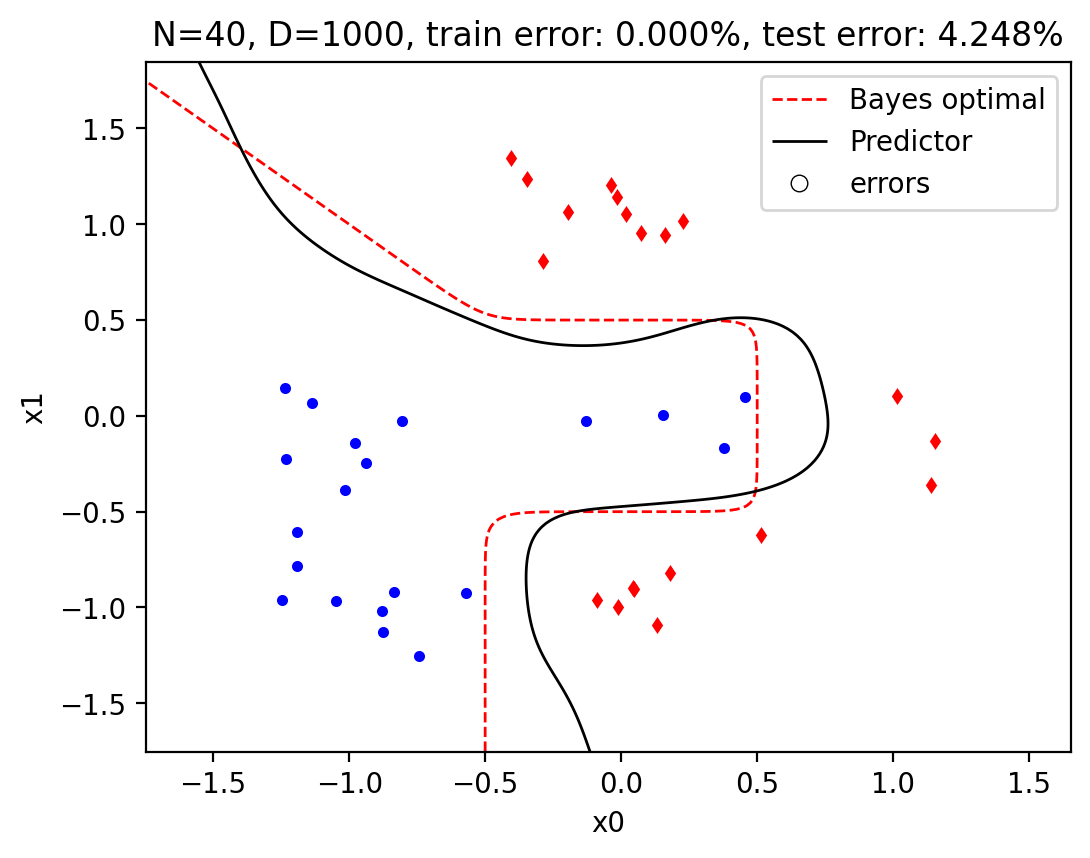
\includegraphics[width=0.8\textwidth]{./images/01_boundary.png}
            \caption*{Classifying points}
        \end{figure}
    \end{minipage}
    \hfill
    \begin{minipage}[b]{0.45\textwidth}
        \begin{figure}
            \centering
            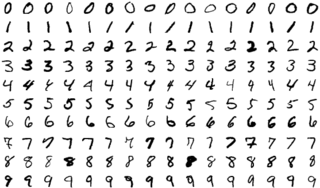
\includegraphics[width=0.8\textwidth]{./images/01_mnist.png}
            \caption*{Classifying images}
        \end{figure}
    \end{minipage}
\end{frame}

\begin{frame}{Tasks by Datasets}
    \begin{block}{Supervised Learning}
        Given a dataset of input-output pairs, learn a function that maps inputs to outputs
        $$\mathcal{T}_m = \left\{\left(x_i, y_i\right) \in \left(\mathcal{X} \times \mathcal{Y}\right)\right\}_{i=1}^{m} \qquad \mathcal{X} \subseteq \mathbb{R}^n$$
    \end{block}
    \begin{block}{Unsupervised Learning}
        Given a dataset of inputs, learn a function that describes the data
        $$\mathcal{T}_m = \left\{x_i \in \mathcal{X}\right\}_{i=1}^{m} \qquad \mathcal{X} \subseteq \mathbb{R}$$
    \end{block}
\end{frame}

\begin{frame}{Supervised Learning}
    \textbf{Classification}
    \begin{itemize}
        \item $y_i \in K$, where $K$ is a set of classes (usually finite)
        \item special case is binary classification, where $K = \left\{0, 1\right\}$ or $K = \left\{-1, 1\right\}$
    \end{itemize}
    \vfill
    \textbf{Regression}
    \begin{itemize}
        \item $y_i \in \mathbb{R}^n$
        \item special case is binary classification, where $K = \left\{0, 1\right\}$ or $K = \left\{-1, 1\right\}$
    \end{itemize}
\end{frame}

\begin{frame}{Mathematical Interlude: Optimisation}
    Neural Networks are trained by \textbf{minimising} a certain \textbf{loss function}

    \vfill

    Now, consider a 1-dimensional function $\mathcal{L}: \mathbb{R} \rightarrow \mathbb{R}$

    \textbf{Analytical solution}

    Using the derivative, we can find all stationary points of the function as
    $$\mathcal{L}^\prime(x) = \frac{d\mathcal{L}}{dx}(x) = 0$$

    Then we have to verify each point wheter it is indeed a minimum
    $$\mathcal{L}^{\prime\prime}(x) = \frac{d^2\mathcal{L}}{dx^2}(x) > 0$$
\end{frame}

\begin{frame}{Mathematical Interlude: Optimisation}
    \textbf{Approximate solution}

    $f^\prime(x_t)$ gives the direction of the tangent to the graph in $x_t$ and thus the direction of the steepest ascent.
    \begin{figure}
        \centering
        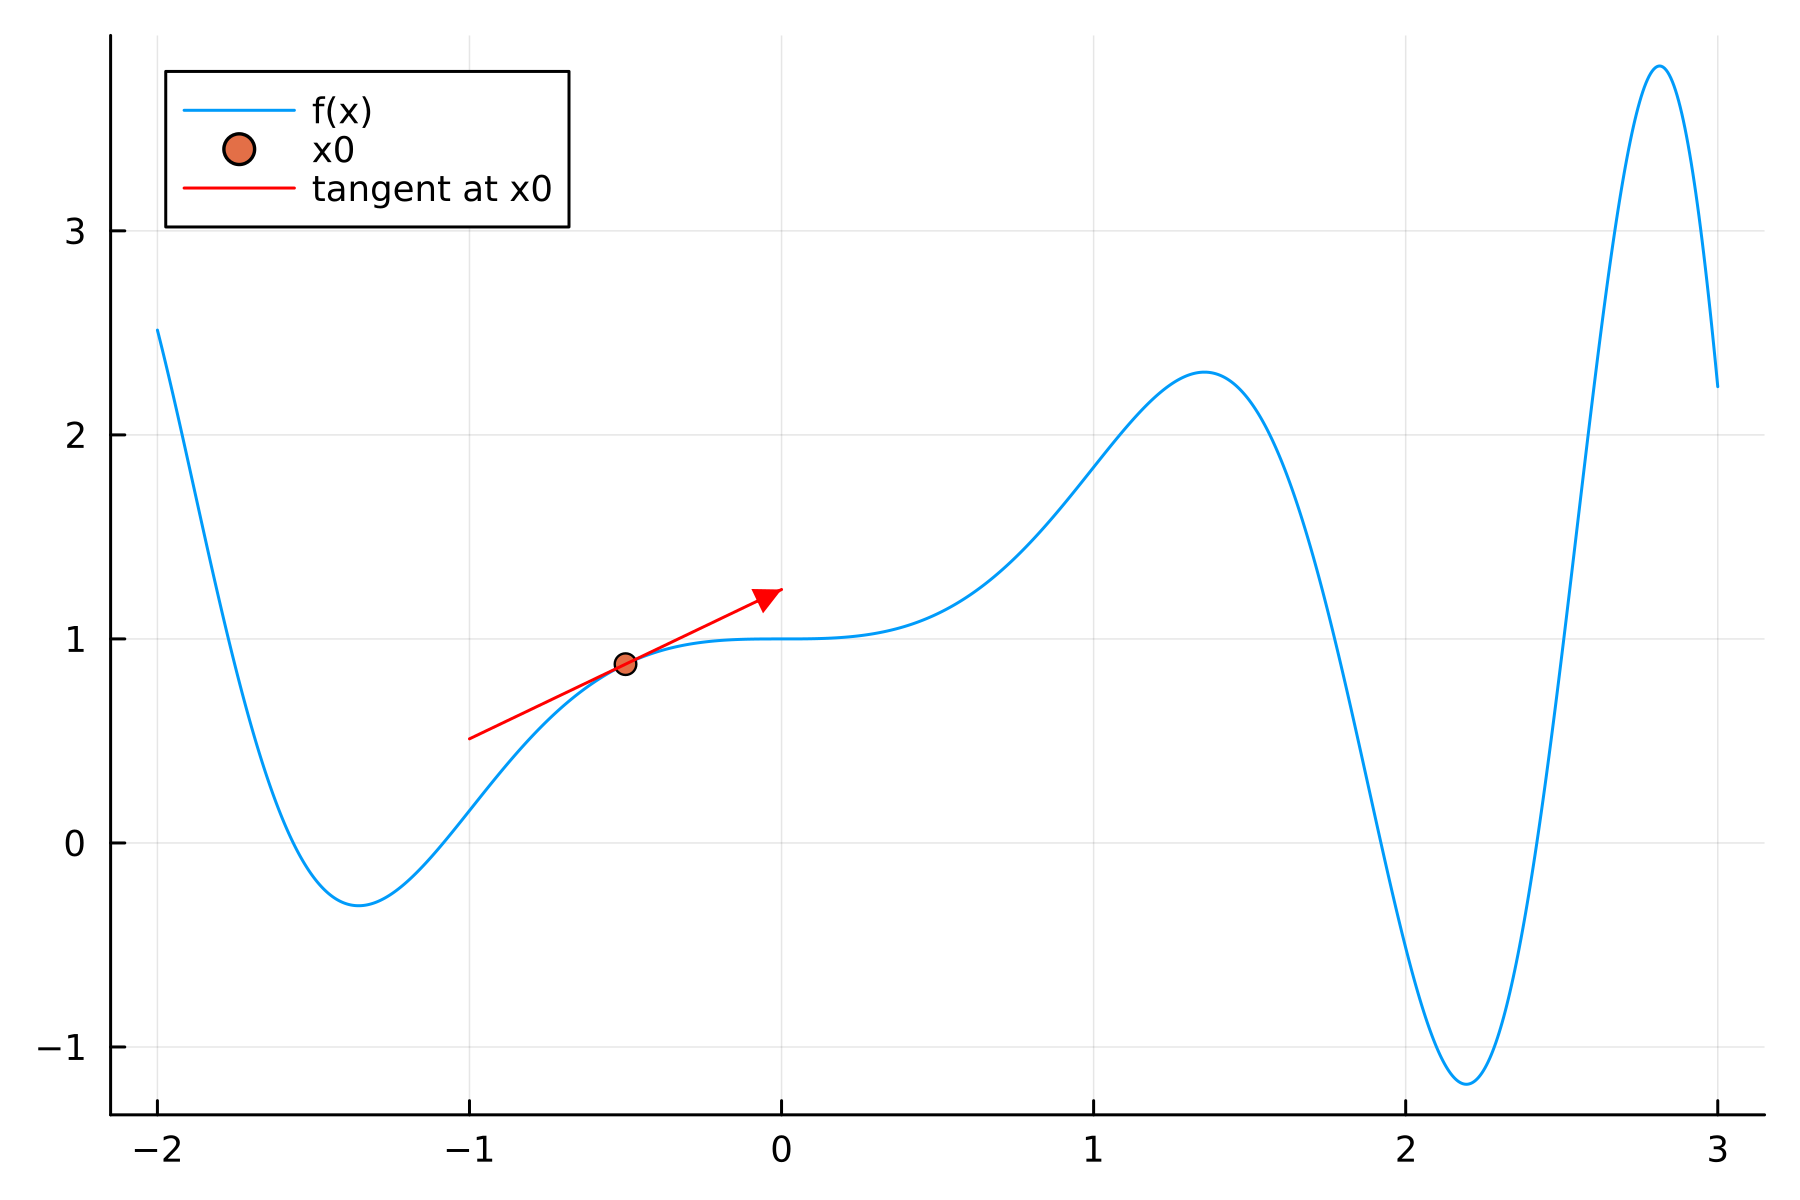
\includegraphics[width=0.4\textwidth]{./images/04_derivative_1d.png}
    \end{figure}
    \begin{block}{Gradient Descent}
        $$x_{t+1} = x_t - \alpha \frac{df}{dx}(x_t) \qquad \alpha \in \left(0, \infty \right]$$
    \end{block}
\end{frame}

\begin{frame}{Mathematical Interlude: Optimisation}

    \begin{minipage}[c]{0.45\textwidth}
        \begin{block}{Point}
            $$x = \left[x_1, \ldots, x_n\right]^T \in \mathbb{R}^n$$
        \end{block}
        \begin{block}{Gradient}
            $$\nabla \mathcal{L} = \left[
                    \frac{\partial \mathcal{L}}{\partial x_1}, \ldots, \frac{\partial \mathcal{L}}{\partial x_n}
                    \right]^T \in \mathbb{R}^n$$
        \end{block}
        \begin{block}{Gradient Descent}
            $$x_{t+1} = x_t - \alpha \nabla \mathcal{L}(x_t)$$
        \end{block}
    \end{minipage}
    \hfill
    \begin{minipage}[c]{0.45\textwidth}
        In reality, loss functions are multi-dimensional $\mathcal{L}: \mathbb{R}^n \rightarrow \mathbb{R}$

        \vfill

        \begin{figure}
            \centering
            \includegraphics<1>[width=\textwidth]{./images/05_function_2d.png}
            \includegraphics<2>[width=\textwidth]{./images/05_contour_2d.png}
        \end{figure}
    \end{minipage}
\end{frame}

\begin{frame}{Mathematical Interlude: Gradient Descent}
    \begin{figure}
        \centering
        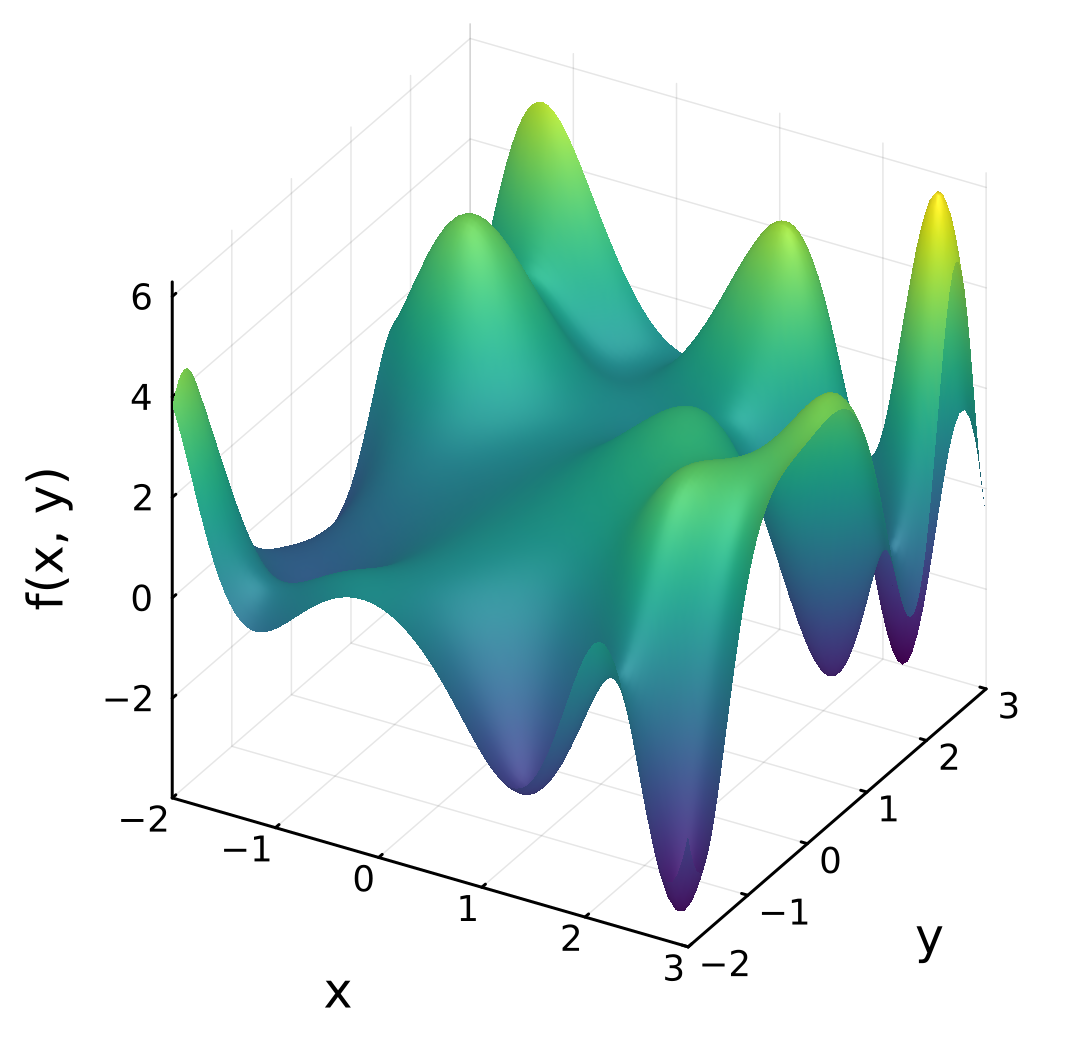
\includegraphics[width=0.6\textwidth]{./images/06_gd_function.png}
    \end{figure}
\end{frame}

\begin{frame}{Mathematical Interlude: Gradient Descent}
    \begin{figure}
        \centering
        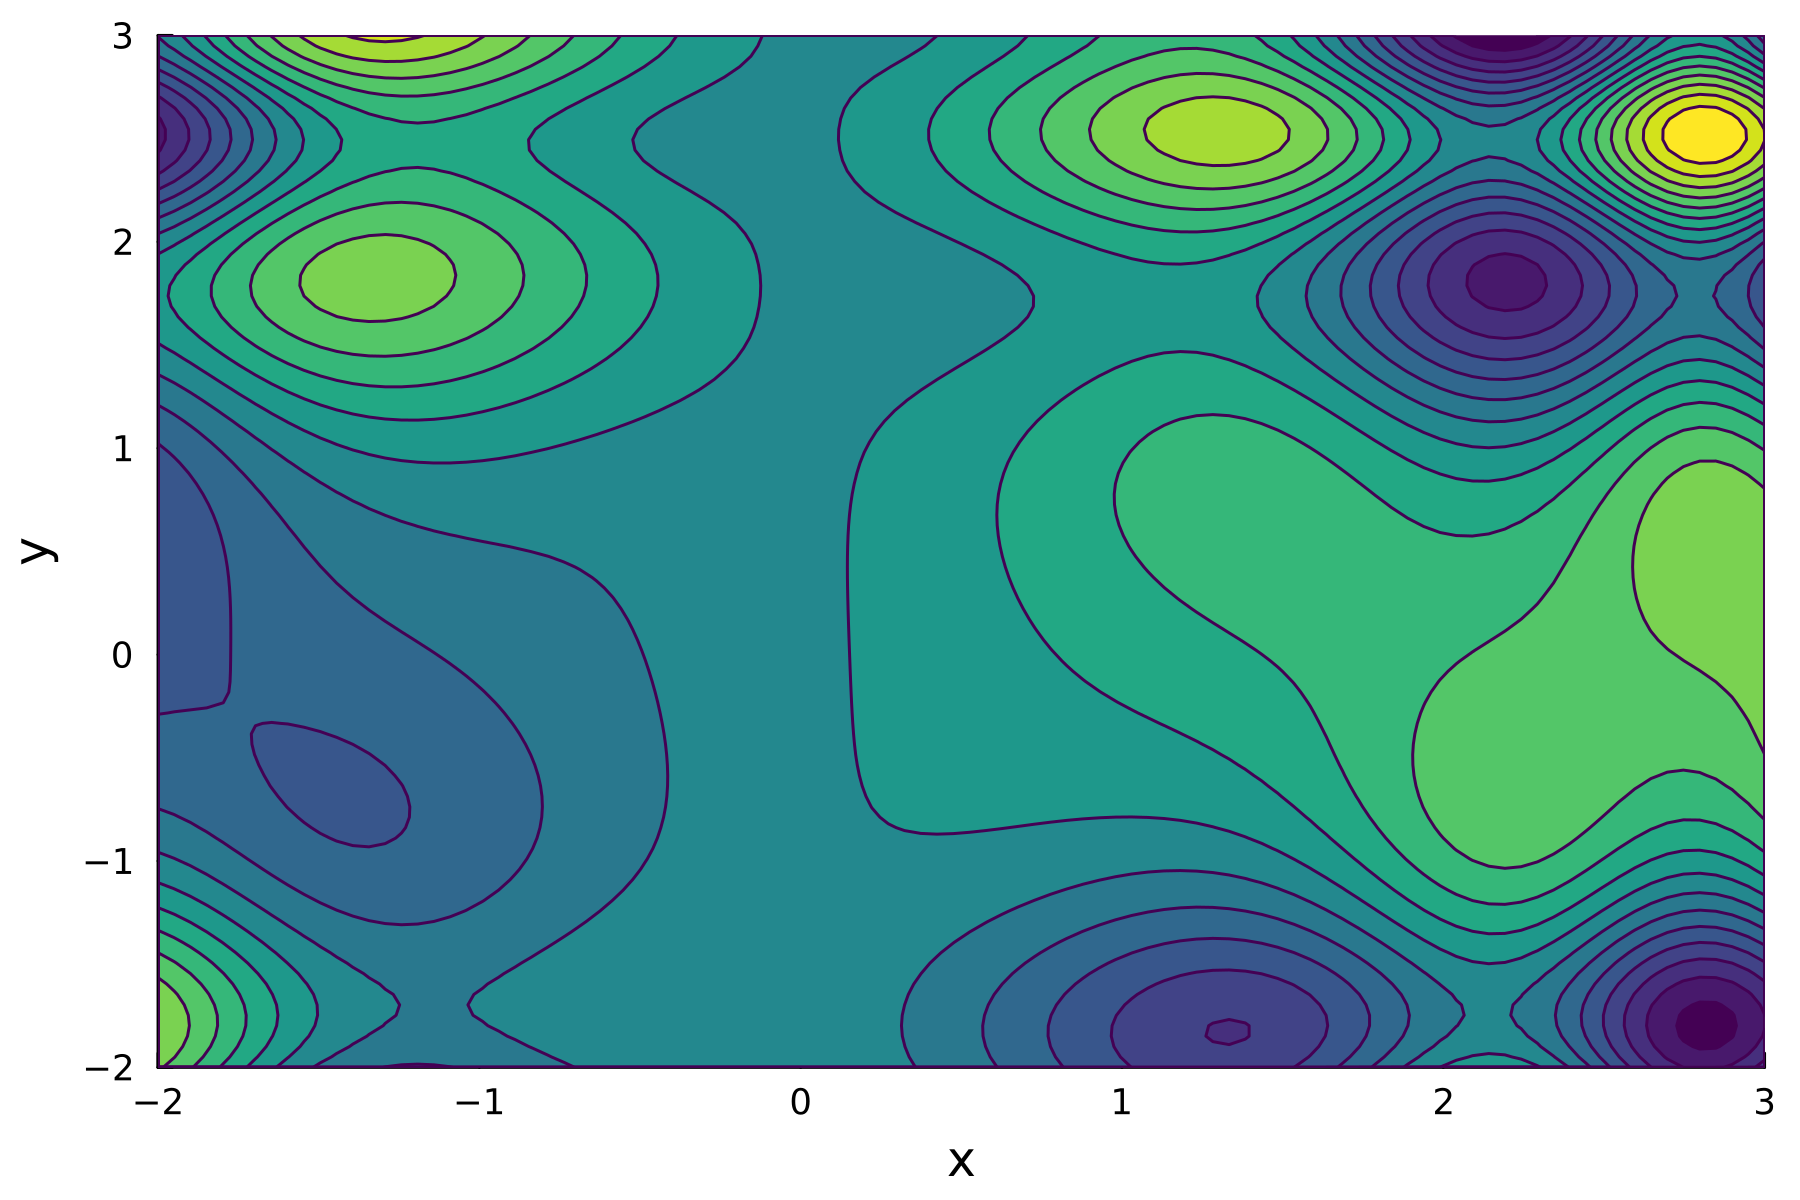
\includegraphics[width=0.9\textwidth]{./images/06_gd_contour.png}
    \end{figure}
\end{frame}

\begin{frame}{Perceptron}
    Consider a simple problem of separating two sets of points in $\mathbb{R}^2$.

    \vfill

    \begin{minipage}{0.45\textwidth}
        \begin{figure}
            \centering
            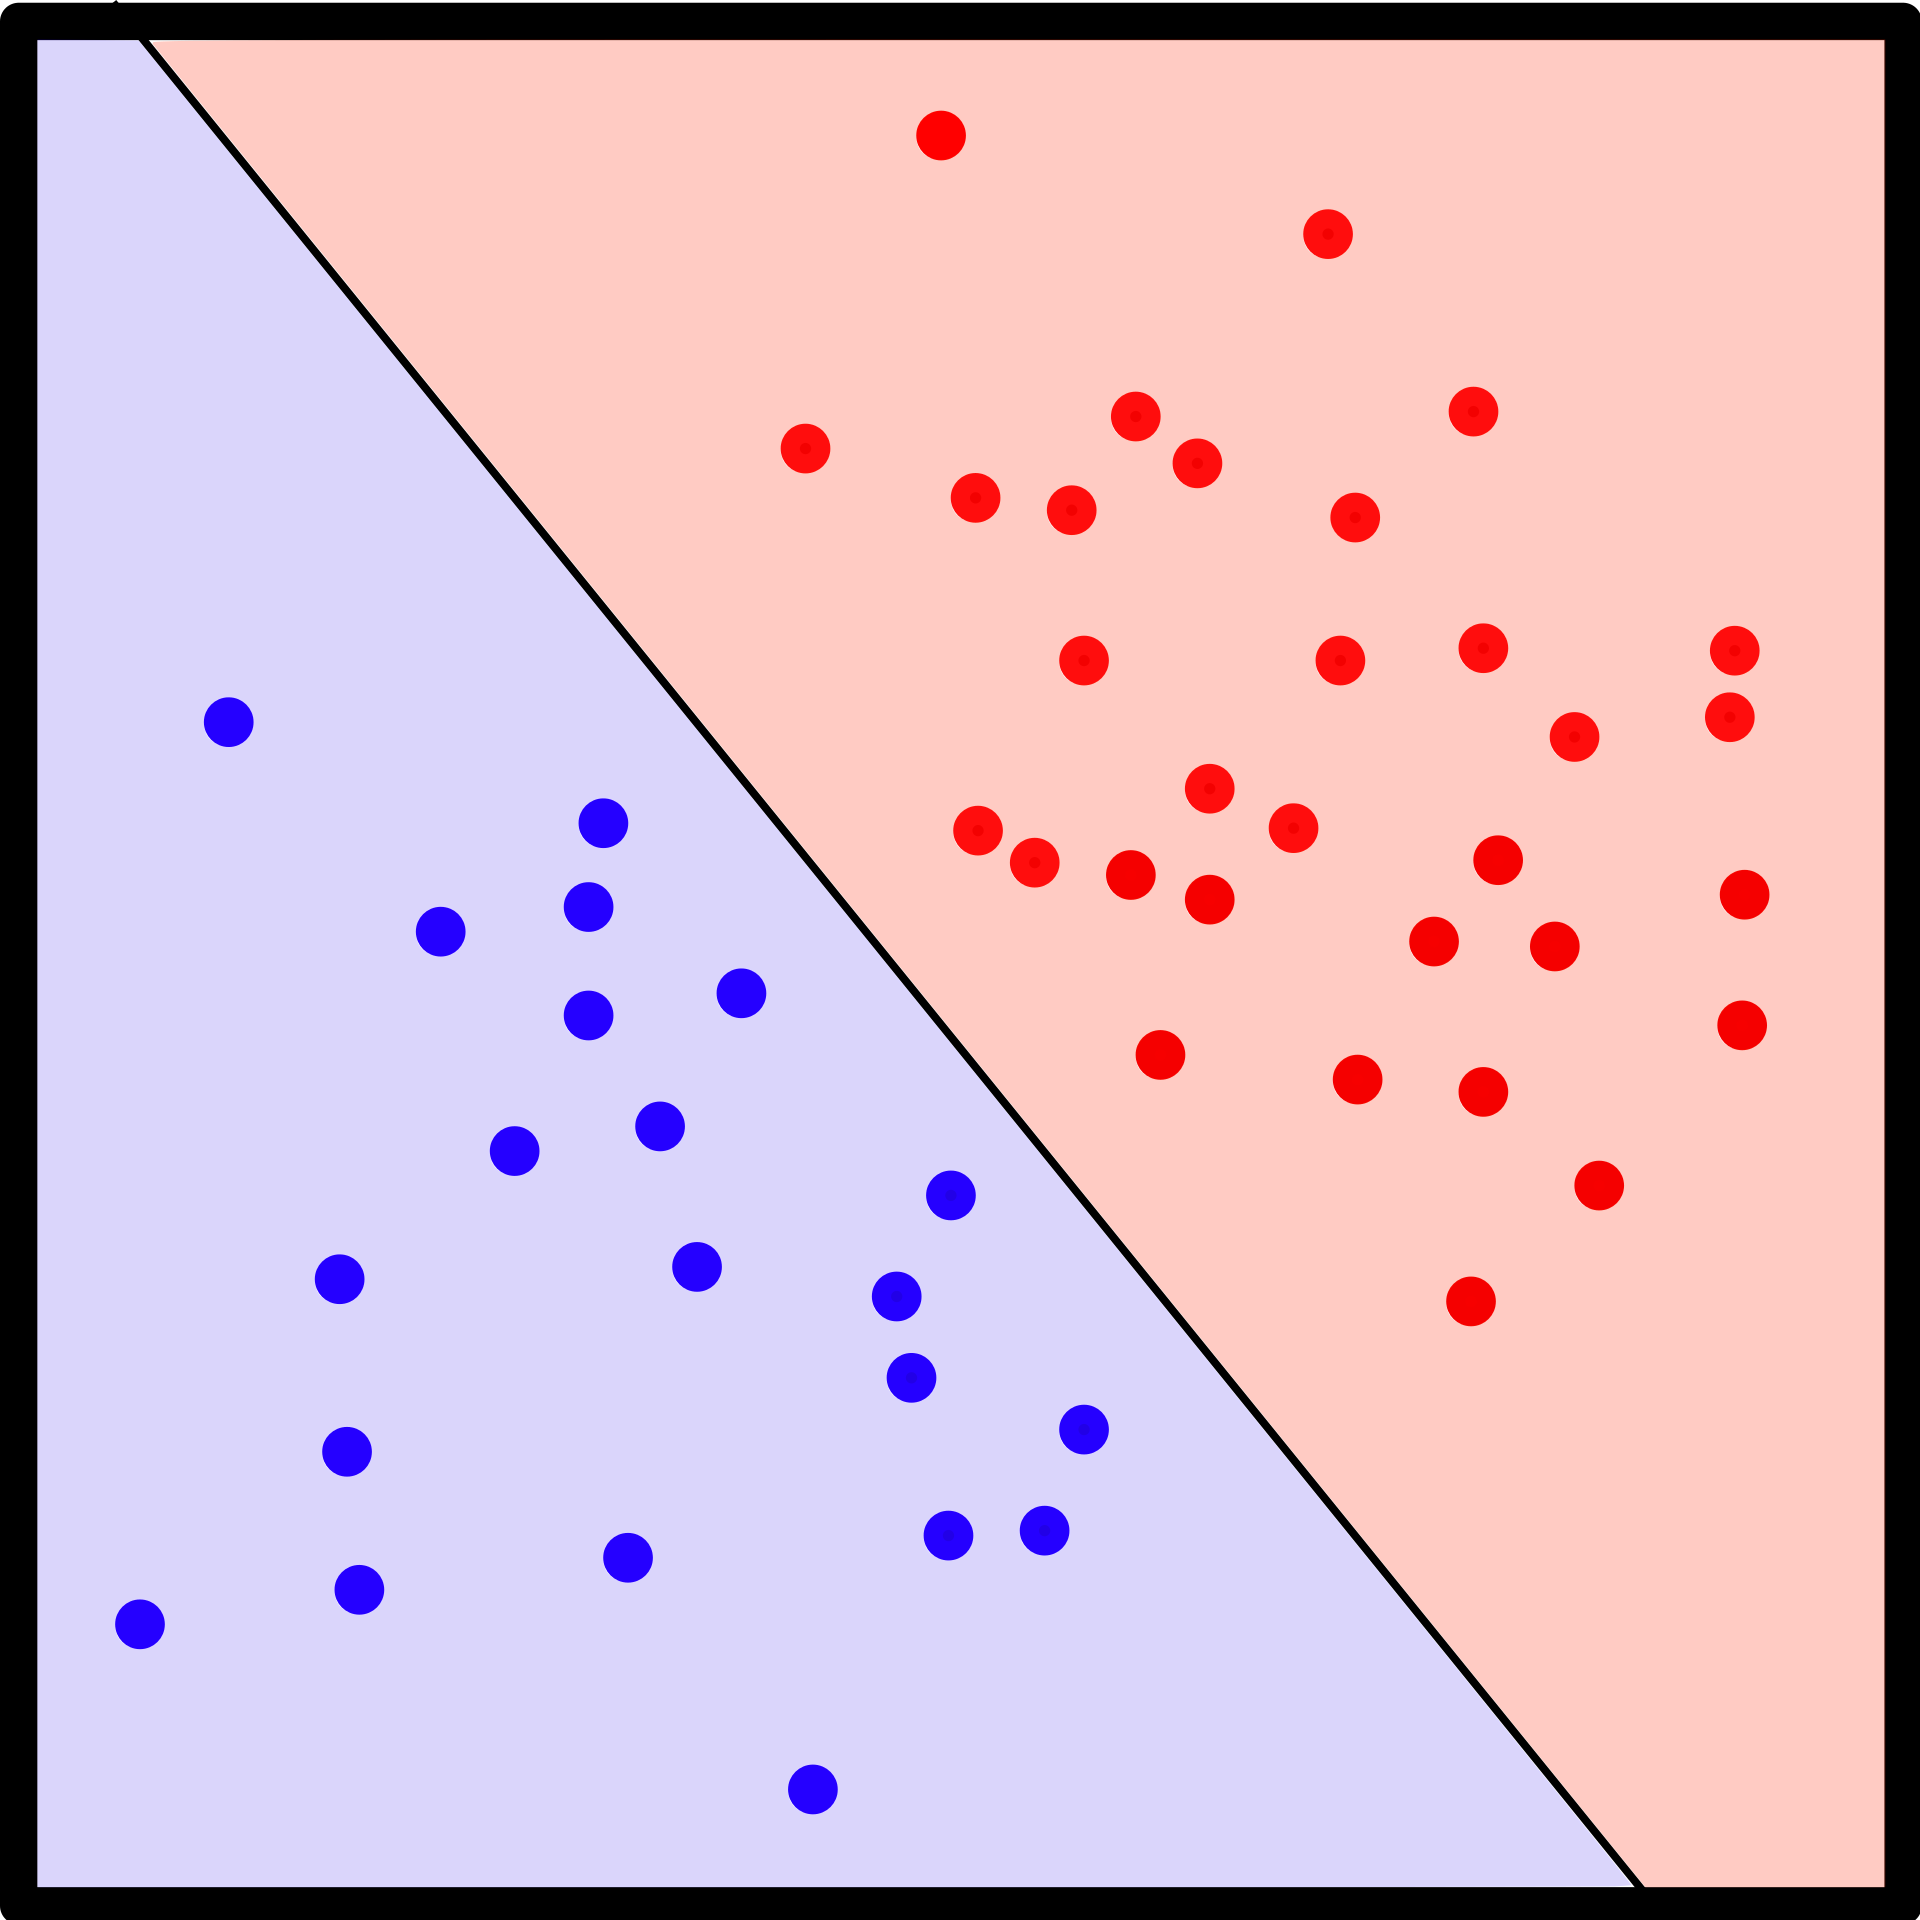
\includegraphics[width=0.8\textwidth]{./images/10_separable_points.png}
        \end{figure}
    \end{minipage}
    \begin{minipage}{0.45\textwidth}
        In this case, it is easy to see that the they can be separated by a line.

        \begin{block}{Normal equation of a line}
            $$\boldsymbol{w}^T\boldsymbol{x} + b = 0$$
        \end{block}
    \end{minipage}

    \vfill

    How can we recognize if a point is above or below the line?
\end{frame}

\begin{frame}{Perceptron: Artificial Neuron}
    $$
        f\left(x\right) = \sign\left(\boldsymbol{w}^T\boldsymbol{x} + b\right) = \begin{cases}
            1  & \text{if } \boldsymbol{w}^T\boldsymbol{x} + b \geq 0 \\
            -1 & \text{if } \boldsymbol{w}^T\boldsymbol{x} + b < 0
        \end{cases}
    $$
    \begin{figure}
        \centering
        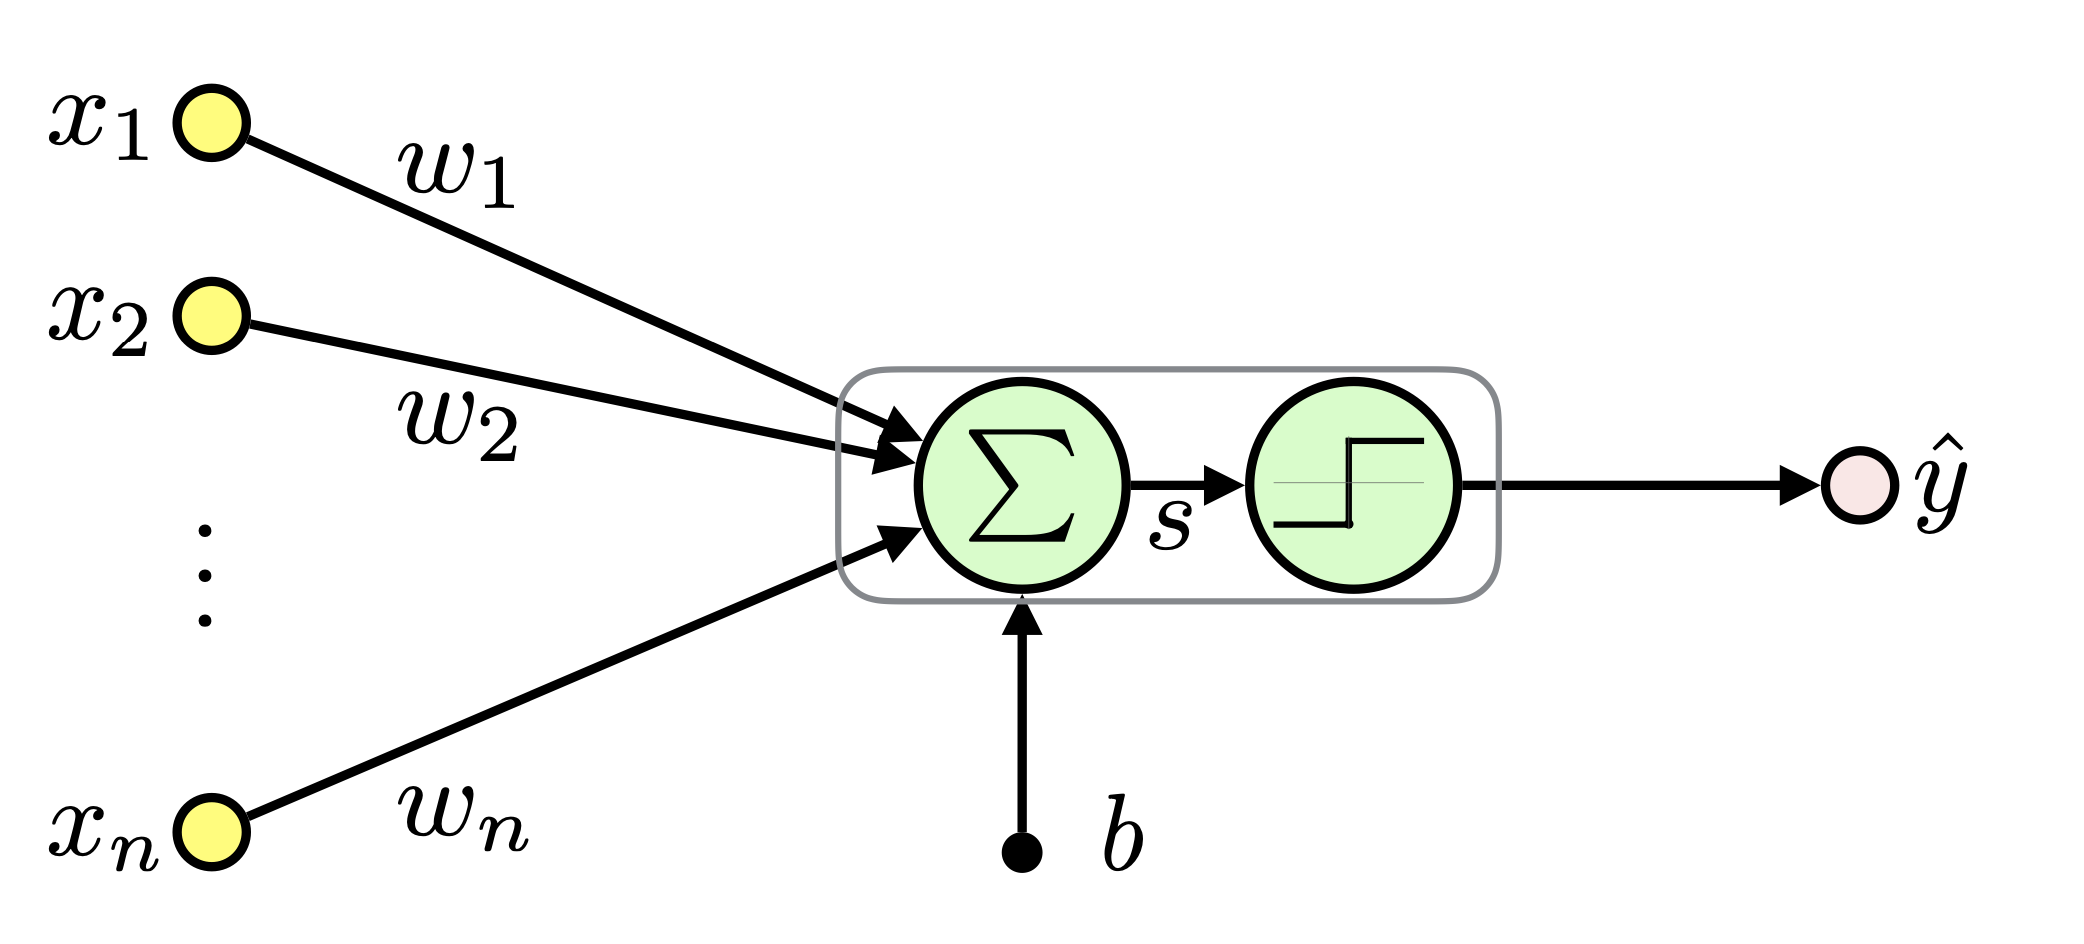
\includegraphics[width=0.5\textwidth]{./images/11_perceptron.png}
    \end{figure}
    Because sign is not good for gradient descent, in Neural Networks we use activation functions that have nice derivatives.
\end{frame}

\begin{frame}{Neural Network}
    In the most basic form, a Neural Network is a collection of neurons aranged into interconnected layers.

    \vfill

    \begin{minipage}{0.45\textwidth}
        \begin{figure}
            \centering
            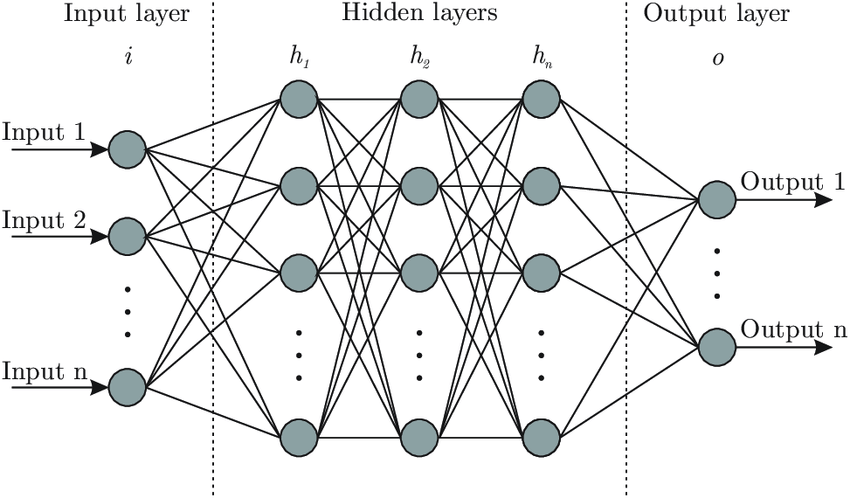
\includegraphics[width=\textwidth]{./images/12_nn.png}
        \end{figure}
    \end{minipage}
    \begin{minipage}{0.45\textwidth}
        \begin{itemize}
            \item Feed-forward NN
            \item Convolutional NN
            \item Recurrent NN
            \item Transformers
            \item ...
        \end{itemize}
    \end{minipage}

    \vfill

    Layers are usually some linear transformation of its inputs followed by an non-linear activation function.
    Another layer (\textit{head}) which transforms the output to a different type of values can be inserted after the last layer.
    At the end is a loss function that defines the task.
\end{frame}

\begin{frame}{Linear (Fully-Connected) Layer}
    A set of neurons that are not connected among themselves. Every input is connected to every neuron, the connection has a learnable weight.

    \vfill

    \begin{minipage}{0.45\textwidth}
        \begin{figure}
            \centering
            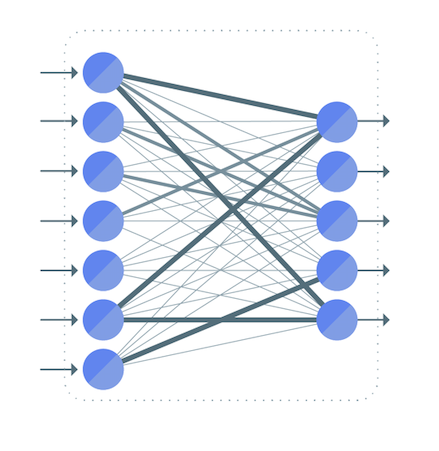
\includegraphics[width=\textwidth]{./images/13_linear_layer.png}
        \end{figure}
    \end{minipage}
    \hfill
    \begin{minipage}{0.45\textwidth}
        \begin{block}{Forward pass}
            $$
                \boldsymbol{y} = \boldsymbol{W}\boldsymbol{x} + \boldsymbol{b}
            $$
            $$
                \boldsymbol{W} \in \mathbb{R}^{m \times n}, \boldsymbol{b} \in \mathbb{R}^m
            $$
        \end{block}
    \end{minipage}
\end{frame}

\begin{frame}{Activations}
    The network needs some nonlinearity so it can approximate other than linear functions $\rightarrow$ \textbf{activation functions}.

    \begin{minipage}[t]{0.3\textwidth}
        \begin{figure}
            \centering
            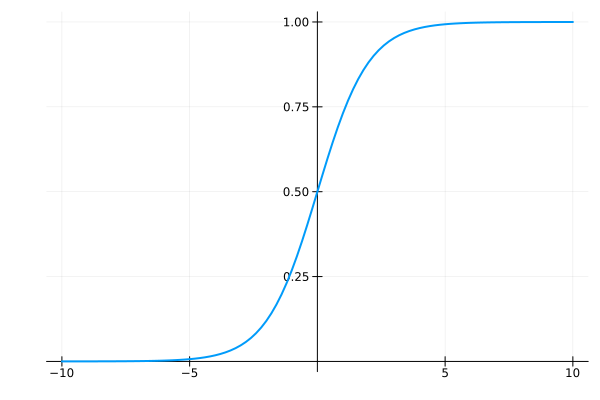
\includegraphics[width=\textwidth]{./images/14_sigmoid.png}
        \end{figure}
        $$\sigma(x) = \frac{1}{1 + e^{-x}}$$
    \end{minipage}
    \hfill
    \begin{minipage}[t]{0.35\textwidth}
        \begin{figure}
            \centering
            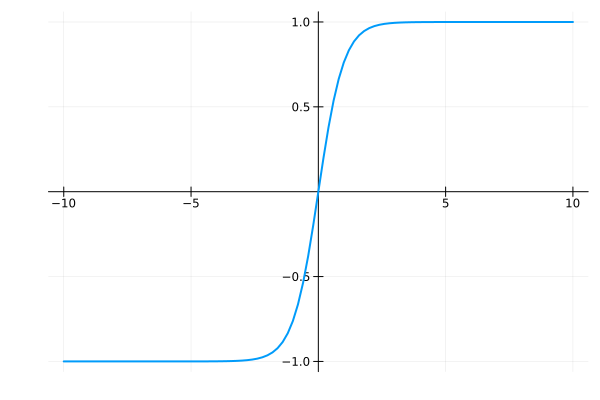
\includegraphics[width=0.86\textwidth]{./images/14_tanh.png}
        \end{figure}
        $$\tanh(x) = \frac{e^x - e^{-x}}{e^x + e^{-x}}$$
    \end{minipage}
    \hfill
    \begin{minipage}[t]{0.3\textwidth}
        \begin{figure}
            \centering
            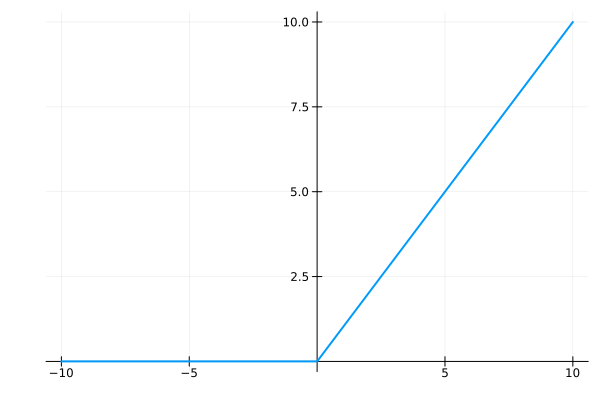
\includegraphics[width=\textwidth]{./images/14_relu.png}
        \end{figure}
        $$\text{ReLU}(x) = \max(0, x)$$
    \end{minipage}

    \vfill

    They work element-wise on the outputs of the neurons of the given layer.
    They are necessary but each of them have different properties.
\end{frame}

\begin{frame}{Softmax}
    Consider \textbf{classification} into $K$ classes and that we would like to predict not only the top class but also the class \textbf{probabilities}.

    \begin{minipage}[t]{0.3\textwidth}
        \begin{figure}
            \centering
            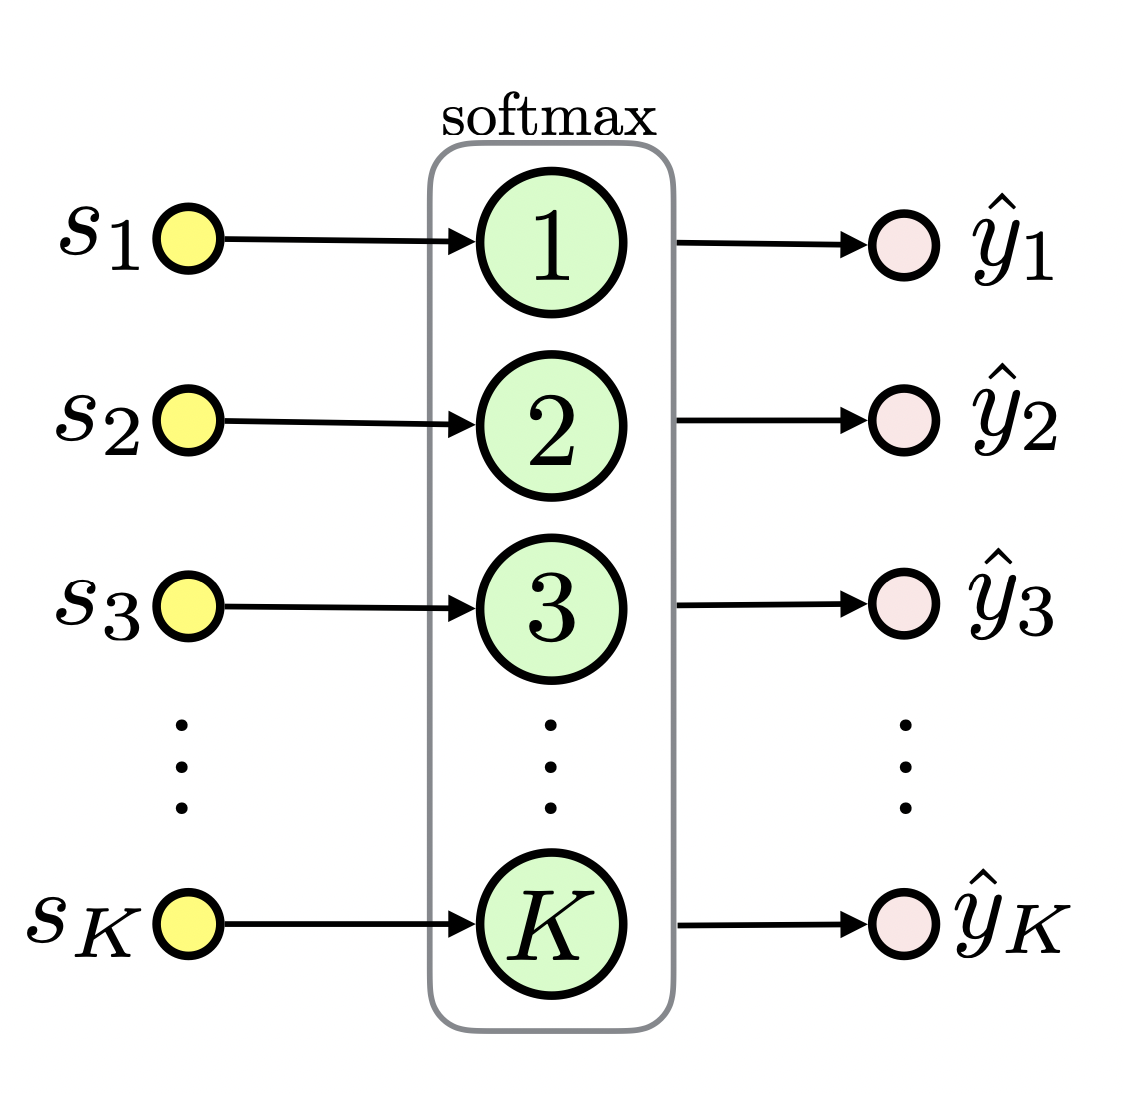
\includegraphics[width=\textwidth]{./images/15_softmax.png}
        \end{figure}
    \end{minipage}
    \hfill
    \begin{minipage}[t]{0.65\textwidth}
        \begin{block}{Softmax}
            $$
                \text{softmax}(\boldsymbol{z})_i = \frac{e^{z_i}}{\sum_{j=1}^{K} e^{z_j}} \qquad i \in \left\{1, \dots, K\right\}
            $$
        \end{block}
    \end{minipage}

    It transforms arbitrary output values into a probability distribution.
    It preserves ordering, so the class with highest predicted value will also have highest proability.
\end{frame}

\begin{frame}{Loss functions}
    Loss function defines the task for which the network is trained.
    Typically, it is a \textbf{scalar} function, i.e. $$\mathcal{L}: \mathbb{R}^n \rightarrow \mathbb{R}$$.

    \vfill

    \textbf{Regression or similar tasks}
    \begin{itemize}
        \item Mean Absolute Error: $\mathcal{L}_{\text{MSE}}(y, y^{\prime}) = ||y - y^{\prime}||_1$
        \item Mean Squared Error: $\mathcal{L}_{\text{MSE}}(y, y^{\prime}) = ||y - y^{\prime}||_2^2$
    \end{itemize}

    \textbf{Classification}
    \begin{itemize}
        \item Negative Log-Likelihood: $\mathcal{L}_{\text{NLL}}(y, y^{\prime}) = -\log(y^{\prime}_y)$ ($y^{\prime}_y$ is the predicted probability of the correct class)
        \item Cross-Entropy: $\mathcal{L}_{\text{CE}}(y, y^{\prime}) = -\sum_{i=1}^{K} y_i \log(y^{\prime}_i)$
    \end{itemize}
\end{frame}

\begin{frame}{Backpropagation}
    As mentioned before, the loss function is optimized by gradient descent using the gradient.
    Thus, we need to compute $\frac{\partial \mathcal{L}}{\partial \theta}$, where $\theta$ are all the weights.

    But how to compute derivative of the loss w.r.t. all the weights?
    \begin{block}{Chain rule}
        Consider composition of functions $f(g(\boldsymbol{x}))$, where $f: \mathbb{R}^m \to \mathbb{R}$ and $g: \mathbb{R}^n \to \mathbb{R}^m$. Then
        $$
            \frac{\partial y}{\partial x_i} = \sum_{k=1}^{m} \frac{\partial y}{\partial u_k} \frac{\partial u_k}{\partial x_i}
        $$
        Note that $\boldsymbol{u} = g(\boldsymbol{x})$ and $y = f(\boldsymbol{u})$.
    \end{block}
\end{frame}

\begin{frame}{Computational Graphs: Basic Example}
    Consider function $\mathcal{L}(a, b, w, t) = ((a + b) \cdot w - t)^2 + w^2$.

    If we know the formula for the loss function, we can compute the derivatives by hand directly.
    \begin{align*}
        \frac{\partial \mathcal{L}}{\partial a} = \frac{\partial L}{\partial b} & = 2((a + b) \cdot w - t) \cdot w            \\
        \frac{\partial \mathcal{L}}{\partial w}                                 & = 2((a + b) \cdot w - t) \cdot (a + b) + 2w \\
        \frac{\partial \mathcal{L}}{\partial t}                                 & = - 2((a + b) \cdot w - t)                  \\
    \end{align*}

    But we can do better.
    Key is to make the process modular and automatic so we do not need to differentiate every loss function from scratch.
\end{frame}

\begin{frame}{Computational Graphs: Basic Example}
    Consider function $\mathcal{L}(a, b, w, t) = ((a + b) \cdot w - t)^2 + w^2$.

    We build a \textbf{computational graph}, i.e. DAG representing the computation.

    \vfill

    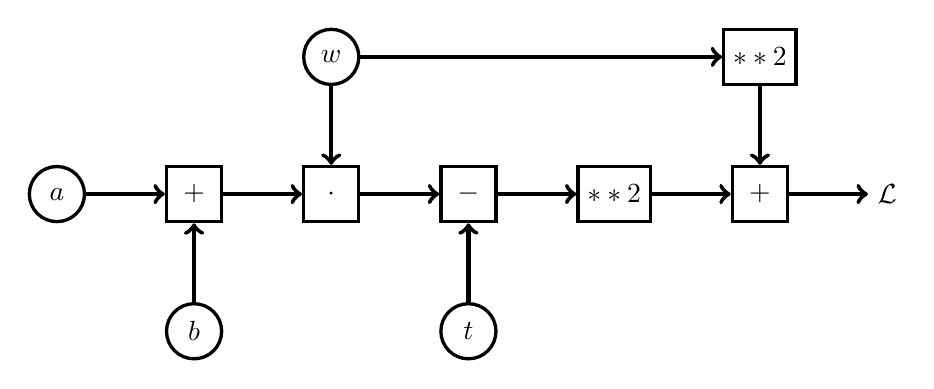
\begin{tikzpicture}[
            roundnode/.style={circle, draw=black, fill=white, very thick, minimum size=7mm},
            squarednode/.style={rectangle, draw=black, fill=white, very thick, minimum size=7mm},
        ]
        \node[roundnode] (a) {$a$};
        \node[squarednode] (plus1) [right=of a] {$+$};
        \node[roundnode] (b) [below=of plus1] {$b$};
        \node[squarednode] (mult1) [right=of plus1] {$\cdot$};
        \node[roundnode] (w) [above=of mult1] {$w$};
        \node[squarednode] (minus) [right=of mult1] {$-$};
        \node[roundnode] (t) [below=of minus] {$t$};
        \node[squarednode] (square1) [right=of minus] {$**2$};
        \node[squarednode] (plus2) [right=of square1] {$+$};
        \node[squarednode] (square2) [above=of plus2] {$**2$};
        \node (loss) [right=of plus2] {$\mathcal{L}$};

        \draw[ultra thick,->] (a) edge (plus1);
        \draw[ultra thick,->] (b) edge (plus1);
        \draw[ultra thick,->] (plus1) edge (mult1);
        \draw[ultra thick,->] (w) edge (mult1);
        \draw[ultra thick,->] (mult1) edge (minus);
        \draw[ultra thick,->] (t) edge (minus);
        \draw[ultra thick,->] (minus) edge (square1);
        \draw[ultra thick,->] (w) edge (square2);
        \draw[ultra thick,->] (square1) edge (plus2);
        \draw[ultra thick,->] (plus2) edge (loss);
        \draw[ultra thick,->] (square2) edge (plus2);
    \end{tikzpicture}
\end{frame}

\begin{frame}{Computational Graphs: Basic Example}
    Now, suppose the current values of parameters are $a=1$, $b=2$, $w=2$, $t=4$.

    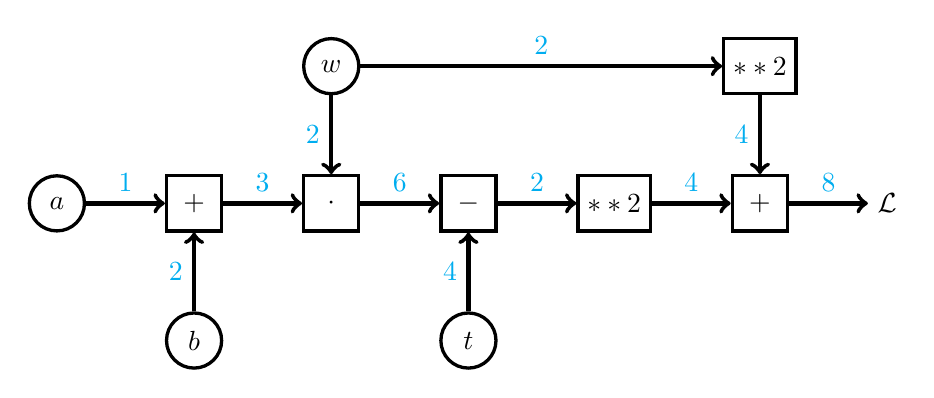
\begin{tikzpicture}[
            roundnode/.style={circle, draw=black, fill=white, very thick, minimum size=7mm},
            squarednode/.style={rectangle, draw=black, fill=white, very thick, minimum size=7mm},
        ]
        \node[roundnode] (a) {$a$};
        \node[squarednode] (plus1) [right=of a] {$+$};
        \node[roundnode] (b) [below=of plus1] {$b$};
        \node[squarednode] (mult1) [right=of plus1] {$\cdot$};
        \node[roundnode] (w) [above=of mult1] {$w$};
        \node[squarednode] (minus) [right=of mult1] {$-$};
        \node[roundnode] (t) [below=of minus] {$t$};
        \node[squarednode] (square1) [right=of minus] {$**2$};
        \node[squarednode] (plus2) [right=of square1] {$+$};
        \node[squarednode] (square2) [above=of plus2] {$**2$};
        \node (loss) [right=of plus2] {$\mathcal{L}$};

        \draw[ultra thick,->] (a) edge node[above,cyan] {1} (plus1);
        \draw[ultra thick,->] (b) edge node[left,cyan] {2} (plus1);
        \draw[ultra thick,->] (plus1) edge node[above,cyan] {3} (mult1);
        \draw[ultra thick,->] (w) edge node[left,cyan] {2} (mult1);
        \draw[ultra thick,->] (mult1) edge node[above,cyan] {6} (minus);
        \draw[ultra thick,->] (t) edge node[left,cyan] {4} (minus);
        \draw[ultra thick,->] (minus) edge node[above,cyan] {2} (square1);
        \draw[ultra thick,->] (w) edge node[above,cyan] {2} (square2);
        \draw[ultra thick,->] (square1) edge node[above,cyan] {4} (plus2);
        \draw[ultra thick,->] (plus2) edge node[above,cyan] {8} (loss);
        \draw[ultra thick,->] (square2) edge node[left,cyan] {4} (plus2);
    \end{tikzpicture}

    We have computed that the value of the loss function is $34$.
    We can verify it by plugging the values into the formula.
    $$
        \mathcal{L}(a, b, w, t) = ((1 + 2) \cdot 2 - 4)^2 + 2^2 = 4 + 4 = 8
    $$
\end{frame}

\begin{frame}{Computational Graphs: Basic Example}
    We can compute the gradients from the loss function and propagate the back through the grap to the leaf nodes.

    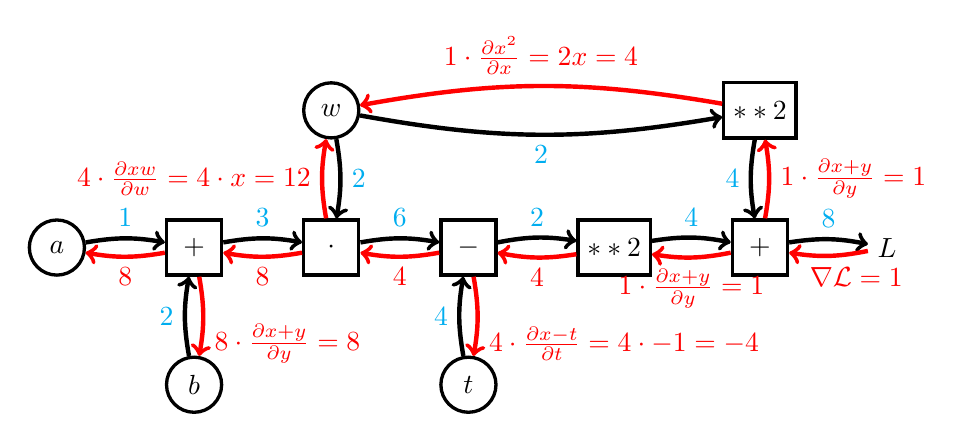
\begin{tikzpicture}[
            roundnode/.style={circle, draw=black, fill=white, very thick, minimum size=7mm},
            squarednode/.style={rectangle, draw=black, fill=white, very thick, minimum size=7mm},
        ]
        \node[roundnode] (a) {$a$};
        \node[squarednode] (plus1) [right=of a] {$+$};
        \node[roundnode] (b) [below=of plus1] {$b$};
        \node[squarednode] (mult1) [right=of plus1] {$\cdot$};
        \node[roundnode] (w) [above=of mult1] {$w$};
        \node[squarednode] (minus) [right=of mult1] {$-$};
        \node[roundnode] (t) [below=of minus] {$t$};
        \node[squarednode] (square1) [right=of minus] {$**2$};
        \node[squarednode] (plus2) [right=of square1] {$+$};
        \node[squarednode] (square2) [above=of plus2] {$**2$};
        \node (loss) [right=of plus2] {$L$};

        \draw[ultra thick,->] (a) edge[auto=right, bend left=10] node[above,cyan] {1} (plus1);
        \draw[ultra thick,->] (plus1) edge[auto=right, bend left=10,red] node[below,red] {$8$} (a);

        \draw[ultra thick,->] (b) edge[auto=right, bend left=10] node[left,cyan] {2} (plus1);
        \draw[ultra thick,->] (plus1) edge[auto=right, bend left=10,red] node[right,red,yshift=-10pt] {$8 \cdot \pd{x + y}{y} = 8$} (b);

        \draw[ultra thick,->] (plus1) edge[auto=right, bend left=10] node[above,cyan] {3} (mult1);
        \draw[ultra thick,->] (mult1) edge[auto=right, bend left=10,red] node[below,red] {$8$} (plus1);

        \draw[ultra thick,->] (w) edge[auto=right, bend left=10] node[right,cyan] {2} (mult1);
        \draw[ultra thick,->] (mult1) edge[auto=right, bend left=10,red] node[left,red] {$4 \cdot \pd{xw}{w} = 4 \cdot x = 12$} (w);

        \draw[ultra thick,->] (mult1) edge[auto=right, bend left=10] node[above,cyan] {6} (minus);
        \draw[ultra thick,->] (minus) edge[auto=right, bend left=10,red] node[below,red] {$4$} (mult1);

        \draw[ultra thick,->] (t) edge[auto=right, bend left=10] node[left,cyan] {4} (minus);
        \draw[ultra thick,->] (minus) edge[auto=right, bend left=10,red] node[right,red,yshift=-10pt] {$4 \cdot \pd{x - t}{t} = 4 \cdot -1 = -4$} (t);

        \draw[ultra thick,->] (minus) edge[auto=right, bend left=10] node[above,cyan] {2} (square1);
        \draw[ultra thick,->] (square1) edge[auto=right, bend left=10,red] node[below,red] {$4$} (minus);

        \draw[ultra thick,->] (w) edge[auto=left, bend right=10] node[below,cyan] {2} (square2);
        \draw[ultra thick,->] (square2) edge[auto=left, bend right=10,red] node[above,red] {$1 \cdot \pd{x^2}{x} = 2x = 4$} (w);

        \draw[ultra thick,->] (square1) edge[auto=right, bend left=10] node[above,cyan] {4} (plus2);
        \draw[ultra thick,->] (plus2) edge[auto=right, bend left=10,red] node[below,red] {$1 \cdot \pd{x + y}{y} = 1$} (square1);

        \draw[ultra thick,->] (plus2) edge[auto=right, bend left=10] node[above,cyan] {8} (loss);
        \draw[ultra thick,->] (loss) edge[auto=right, bend left=10,red] node[below,red,xshift=10pt] {$\nabla \mathcal{L} = 1$} (plus2);

        \draw[ultra thick,->] (square2) edge[auto=left, bend right=10] node[left,cyan] {4} (plus2);
        \draw[ultra thick,->] (plus2) edge[auto=left, bend right=10,red] node[right,red] {$1\cdot\pd{x + y}{y} = 1$} (square2);

    \end{tikzpicture}
\end{frame}

\begin{frame}{Computational Graphs: Basic Example}
    We can verify the gradients by computing them by hand.

    \vfill

    \begin{align*}
        \frac{\partial \mathcal{L}}{\partial a} = \frac{\partial L}{\partial b} & = 2((1 + 2) \cdot 2 - 4) \cdot 2  = 8                   \\
        \frac{\partial \mathcal{L}}{\partial w}                                 & = 2((1 + 2) \cdot 2 - 4) \cdot (1 + 2) + 2 \cdot 2 = 16 \\
        \frac{\partial \mathcal{L}}{\partial t}                                 & = - 2((1 + 2) \cdot 2 - 4) = -4                         \\
    \end{align*}
\end{frame}

\begin{frame}{Computational Graphs: Neural Networks}
    The modules can be arbitrarily granular, i.e. a whole layer can be a single node in the computational graph.

    \begin{figure}[ht]
        \centering
        \includegraphics<1>[width=0.5\textwidth]{./images/22_backprop_module.png}
        \includegraphics<2>[width=0.9\textwidth]{./images/22_backprop_nn.png}
    \end{figure}

    It is sufficient to define \textbf{forward} and \textbf{backward} methods for each such module.
\end{frame}

\begin{frame}{Stochastic Gradient Descent}
    In plain Gradient Descent, the gradient is computed on the whole dataset.
    For big datasets, this can take a very long time to make a small step.

    \textbf{Stochastic Gradient Descent} makes a single step on a small subset of the whole dataset.
    We sample a mini-batch $I = \left\{i_1, \dots, i_M\right\}$ of size $M$ at random without replacement and estimate the true gradient by
    $$\tilde{g} = \frac{1}{M}\sum_{i \in I}\nabla l_i(\theta_t)$$
    The gradient update is then
    $$\theta_{t+1} = \theta_{t} - \alpha \tilde{g}$$
\end{frame}

\begin{frame}{Stochastic Gradient Descent}
    \begin{figure}
        \centering
        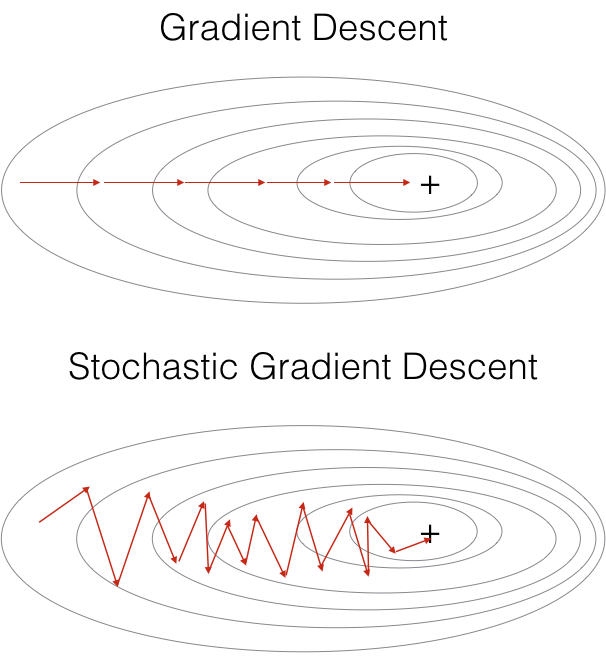
\includegraphics[width=0.5\textwidth]{./images/24_sgd.png}
    \end{figure}
\end{frame}

\end{document}
